\documentclass{ctexart}
\usepackage{graphicx}
\usepackage{amsmath}
\usepackage{bm}
\usepackage{xcolor}
\begin{document}
	\section{凸集}
	
	\subsection{仿射集合和凸集}
	
	\textbf{直线和线段}
	
	设\(x_1 \neq x_2\)为\(R^n\)空间中的两个点,具有如下形式:
	
	\[y = \theta x_1 + (1-\theta)x_2, \theta \in R\]
	
	组成一条穿越\(x_1, x_2\)的直线。参数\(\theta=0\)对应\(y = x_2\),而\(\theta=1\)表明\(y = x_1\)。
	
	参数\(\theta\)的值在0和1之间波动,构成了\(x_1, x_2\)之间的(闭)线段。
	
	y的表示形式:
	
	\[y = x_2 + \theta(x_1-x_2)\]
	
	另一种解释:y是基点\(x_2\)(对应\(\theta=0\))和方向(\(x_1-x_2\))(由\(x_2\)指向\(x_1\))乘以参数\(\theta\)的和。因此\(\theta\)给出了y在由\(x_2\)通向\(x_1\)的路上的位置。当\(\theta\)由0增加到1,点y相应地由\(x_2\)移动到\(x_1\)。如果\(\theta > 1\),点y在超越了\(x_1\)的直线上。如下图所示:
	
	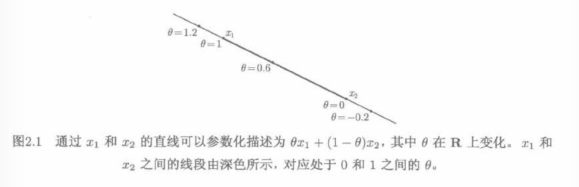
\includegraphics[width=1\linewidth]{pic/pic2_1}
	
	\mbox{}
	
	\textbf{仿射集合}
	
	如果通过集合\(C \subseteq R^N\)中任意两个不同点的{\color{red}直线}仍然在集合C中,那么称集合C是仿射的。也就是说,\(C \subseteq R^N\)是仿射等价于:对于任意\(x_1,x_2 \in C, \theta \in R\)有\(\theta x_1 + (1-\theta)x_2 \in C\)。换而言之,C包含了C中任意两点的系数之和为1的线性组合。
	
	\textbf{ATTENTION!}这里并没有限制\(\theta\)的大小,也就是说经过两点的直线仍在C中。
	
	扩展到多个点。如果\(\theta_1 + ··· +\theta_k = 1\),称具有\(\theta_1 x_1 + ··· +\theta_k x_k\)形式的点为\(x_1,...,x_k\)的仿射组合。
	
	结论:一个仿射集合包含其中任意点的仿射组合,如果C是一个仿射集合,\(x_1,...,x_k \in C, \theta_1 + ... + \theta_k = 1\),那么\(\theta_1 x_1 + ··· +\theta_k x_k\)仍然在C中。
	
	如果C是一个仿射集合且\(x_0 \in C\),则集合
	
	\[V = C-x_0 = \{x-x_0|x\in C\}\]
	
	是一个子空间,即关于加法和数乘是封闭的。
	
	设\(v_1,v_2 \in V, \alpha, \beta \in R\)则有\(v_1 + x_0 \in C, v_2 + x_0 \in C\),因为C是仿射的,且\(\alpha + \beta + (1-\alpha - \beta) = 1\),所以
	
	\[\alpha v_1 + \beta v_2 + x_0 = \alpha(v_1 + x_0) + \beta(v_2 + x_0) + (1-\alpha - \beta)x_0 \in C\]
	
	由\(\alpha v_1 + \beta v_2 + x_0 \in C\),可知\(\alpha v_1 + \beta v_2 \in V\)
	
	因此仿射集合C可以表示为:
	
	\[C = V + x_0 = \{v + x_0|v \in V\}\]
	
	即一个子空间加上一个偏移。与仿射集合C相关联的子空间V与\(x_0\)的选取无关,所以\(X_0\)可以是C中的任意一点。
	
	我们定义仿射集合C的维数为子空间\(V = C - x_0\)的维数,其中\(x_0\)是C中的任意元素
	
	我们称由集合\(C \subseteq R^n\) 中的点所有仿射组合组成的集合为C的仿射包,记为aff C:
	
	\[aff C = \{\theta_1 x_1+ ··· + \theta_k x_k|x_1,...,x_k \in C, \theta_1+···+\theta_k=1\}\]
	
	仿射包是包含C的最小的仿射集合,也就是说:如果S是满足\(C \subseteq S\)的仿射集合,那么\(aff C \subseteq S\)
	
	\textbf{仿射维数与相对内部}
	
	我们定义集合C的仿射维数为其仿射包的维数。
	
	如果集合\(C \subseteq R^n\)的仿射维数小于n,那么这个集合在仿射集合\(aff C \neq R^n\)中。我们定义集合C的相对内部为aff C的内部,记为relint C,即
	
	\[relint C = \{x \in C|B(x, r) \cap aff C \subseteq C for  some  r > 0\}\]
	
	其中\(B(x, r) = \{y| ||y-x|| \leq r\}\)即半径为r,中心为x并由范数||·||定义的球。
	
	我们定义集合C的相对边界为cl C\\relint C,此处cl C表示C的闭包
	
	\textbf{凸集}
	
	集合C被称为凸集,如果C中任意两点间的{\color{red}线段}仍然在C中,即对任意\(x_1, x_2 \in C\)和满足\(0 \leq \theta \leq 1\)的\(\theta\)都有
	
	\[\theta x_1 + (1-\theta)x_2 \in C\]
	
	如果集合中的没一点都可以被其他点沿着他们之间一条无阻碍的路径看见,那么这个集合就是凸集。所谓无阻碍,是指整条路径都在集合中。由于仿射集合包含穿过集合中任意不同两点的整条直线,任意不同两点间的线段自然也在集合中。{\color{red}因而仿射集是凸集。}
	
	我们称点\(\theta_1x_1 + ...+\theta_kx_k\)为点\(x_1,...,x_k\)的一个凸组合,其中\(\theta_1+...+\theta_k = 1, \theta_i \geq 0, i = 1,...,k\),一个集合是凸集等价于集合包含其中所有点的凸组合。
	
	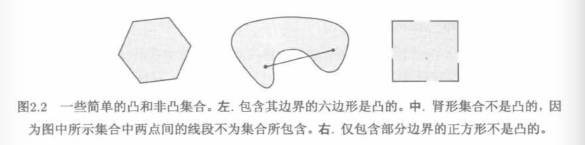
\includegraphics[width=1\linewidth]{pic/pic2_2}
	
	我们称集合C中所有点的凸组合的集合为其凸包,记为conv C:
	
	\[conv C = \{\theta_1 x_1 + ···+\theta_k x_k|x_i \in C, \theta_i \geq 0, i =1,..,k, \theta_1+...+\theta_k=1\}\]
	
	凸包conv C总是凸的。它是包含C的最小的凸集。也就是说,如果B是包含C的凸集,那么\(conv C \subseteq B\)
	
	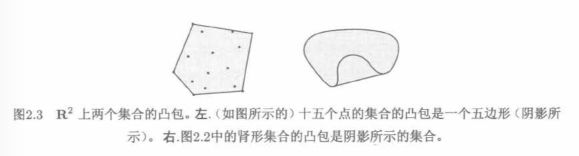
\includegraphics[width=1\linewidth]{pic/pic2_3}
	
	\textbf{锥}
	
	如果对于任意\(x \in C, \theta \geq 0\)都有\(\theta x \in C\),我们称集合C是锥或者是非负齐次。如果集合C是锥,并且是凸的,则称C为凸锥,对于任意\(x_1, x_2 \in C, \theta_1, \theta_2 \geq 0\)都有
	
	\[\theta_1 x_1 + \theta_2 x_2 \in C\]
	
	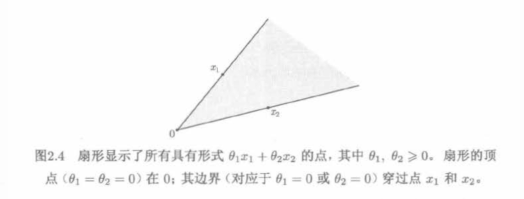
\includegraphics[width=1\linewidth]{pic/pic2_4}
	
	具有\(\theta_1 x_1 + ··· + \theta_k x_k, \theta_1,...,\theta_k \geq 0\)形式的点成为\(x_1,...x_k\)的锥组合(非负线性组合)
	
	集合C的锥包是C中元素的所有锥组合的集合,即:
	
	\[\{\theta_1 x_1 +····+ \theta_k x_k|x_i \in C, \theta_i \geq 0, i =1,...,k\}\]
	
	它是包含C的最小的凸锥
	
	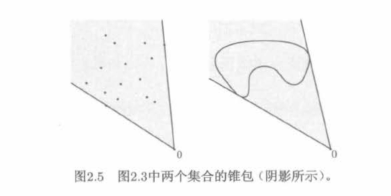
\includegraphics[width=1\linewidth]{pic/pic2_5}
	
	\subsection{重要的例子}
	
	\textbf{超平面与半空间}
	
	超平面是具有以下形式的集合
	
	\[\{x|a^Tx=b\}\]
	
	其中\(a \in R^n, a \neq 0, b \in R\).超平面是关于x的非平凡线性方程的解空间(因此是一个仿射集合)。几何上,超平面可以解释为与给定向量a的内积为常数的点的集合;也可以看成法线方向为a的超平面,而常数\(b \in R\)决定了这个平面从原点的偏移。
	
	超平面还可以表示成如下形式:
	
	\[\{x|a^T(x-x_0)=0\}\]
	
	其中\(x_0\)是超平面上的任意一点。	
	
	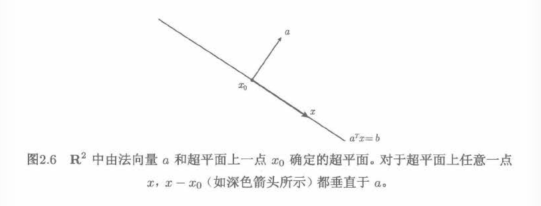
\includegraphics[width=1\linewidth]{pic/pic2_6}
	
	一个超平面将\(R^n\)划分为两个半空间。半空间有如下形式:
	
	\[\{x|a^Tx \leq b\}\]
	
	即非平凡的线性不等式的解空间。其中\(a \neq 0\).半空间是凸的,但不是仿射的。
	
	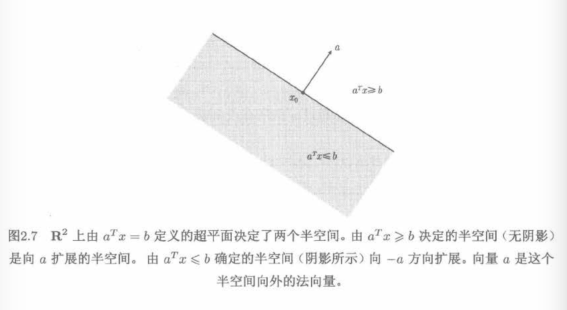
\includegraphics[width=1\linewidth]{pic/pic2_7}
	
	半空间也可以表示为
	
	\[\{x|a^T(x-x_0) \leq 0\}\]
	
	几何解释:半空间由\(x_0\)加上任意与(向外的法)向量a呈钝角的向量组成 
	
	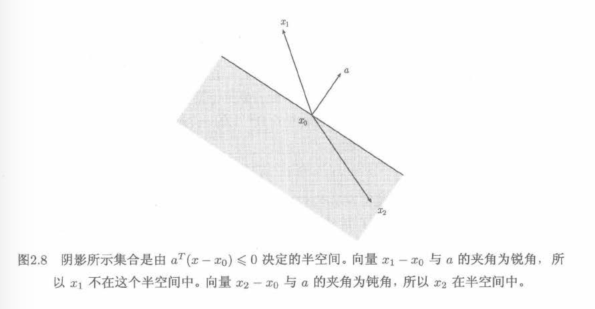
\includegraphics[width=1\linewidth]{pic/pic2_8}
	
	\textbf{Euclid球和椭球}
	
	\(R^n\)中的空间Euclid球,具有以下形式:
	
	\[B(x_c, r)=\{x | ||x-x_c||_2 \leq r\}=\{x|(x-x_c)^T(x-x_c) \leq r^2\}\]
	
	其中r>0, \(||·||_2\)表示Euclid范数,即\(||u||_2=(u^Tu)^{1/2}\),向量\(x_c\)是球心,标量r为半径。\(B(x_c, r)\)由距离球心\(x_c\)距离不超过r的所有点组成。另一个常见的表达式为,
	
	\[B(x_c, r)=\{x_c+ru| \parallel u\parallel_2 \leq 1\}\]
	
	一类相关的凸集是椭球,具有如下形式:
	
	\[\varepsilon = \{x|(x-x_c)^TP^{-1}(x-x_c) \leq 1\}\]
	
	其中\(P=P^T \succ 0\),即P使对称正定矩阵。向量\(x_c \in R^n\)为椭球的中心。矩阵P决定了椭球从\(x_c\)向各个方向扩展的幅度。\(\varepsilon\)的半轴长度由\(\sqrt{\lambda_i}\)给出,\(\lambda_i\)为P的特征值。球可以看成是\(P=r^2I\)的椭球。
	
	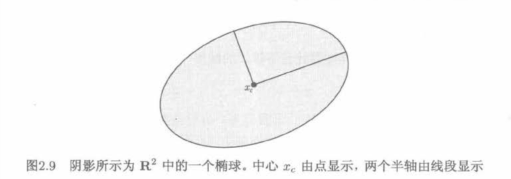
\includegraphics[width=1\linewidth]{pic/pic2_9}
	
	椭球另一个常用的表示形式
	
	\[\varepsilon = \{x_c+Au| \parallel u \parallel_2 \leq 1\}\]
	
	其中A是非奇异的方阵。
	
	设\(\parallel · \parallel\)是\(R^n\)中的范数。由范数的一般性质知,以r为半径,\(x_c\)为球心的范数球\(\{x| \parallel x-x_c\parallel \leq r\}\)是凸的。
	
	关于范数\(\parallel · \parallel\)的范数锥是集合
	
	\[C = \{(x,t)| \parallel x\parallel \leq t\} \subseteq R^{n+1}\]
	
	是一个凸锥
	
	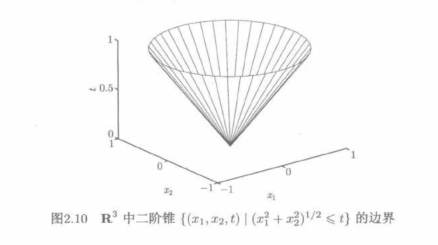
\includegraphics[width=1\linewidth]{pic/pic2_10}
	
	\textbf{多面体}
	
	多面体被定义为有限个线性等式和不等式的解集
	
	\[P = \{a_j^Tx \leq b_j, j = 1,...,m, c_j^Tx=d_j, j=1,...,p\}\]
	
	因此多面体是有限个半空间和超平面的交集。
	
	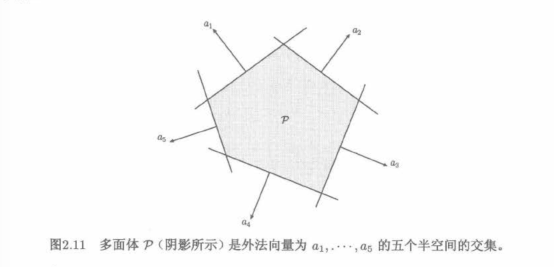
\includegraphics[width=1\linewidth]{pic/pic2_11}
	
	单纯形是一类重要的多面体。设k+1个点\(v_0,..,v_k \in R^n\)仿射独立,即\(v_1-v_0,...,v_k-v_0\)线性独立,那么这些点决定了一个单纯形,如下
	
	\[C = conv\{v_0,...,v_k\}=\{\theta_0v_0+...+\theta_kv_k| \theta \succeq 0, \bm{1}^T\theta = 1\}\]
	
	其中\(\bm{1}\)表示所有分量均为一的向量。这个单纯形的仿射维数为k,因此也成为\(R^n\)空间的k维单纯形。
	
	\textbf{思考:}\(\{\theta_0v_0+...+\theta_kv_k| \theta \succeq 0, \bm{1}^T\theta = 1\}\)这一串其实就是凸集的定义吧,\(\theta \succeq 0\)其实就是向量\(\theta\)的\(\theta_i \geq 0\), \(\bm{1}^T\theta = 1\)就是\(\theta_0+···+\theta_k = 1\)
	所以\(\theta \succeq 0, \bm{1}^T\theta = 1\),有\(x=\theta_0v_0+\theta_1v_1+...+\theta_kv_k\).
	
	如果定义\(y=(\theta_1,...,\theta_k)\)和
	
	\[B = [v_1-v_0 ··· v_k-v_0] \in R^{n\times k}\]
	
	\(x \in C\)的充要条件是
	
	\[x = v_0 + By\]	
	
	对于\(y \succeq 0, \bm{1}^Ty \leq 1\)成立
	
	\begin{align*}
	x & = v_0 + By = v_0 + (v_1-v_0)\theta_1+...+(v_k-v_0)\theta_k \\
	   & = v_0 + v_1\theta_1 +....+ v_k\theta_k - (\theta_1+....+\theta_k)v_0 \\
	   & =v_0\theta_0 - v_0\theta_0 + v_0 + v_1\theta_1 +....+ v_k\theta_k - (\theta_1+....+\theta_k)v_0 \\
	   & =(v_0\theta_0+v_1\theta_1+...+v_k\theta_k) + v_0 - (\theta_0+...+\theta_k)v_0 \\
	   & = (v_0\theta_0+v_1\theta_1+...+v_k\theta_k) + v_0 -v_0 \\
	   & = (v_0\theta_0+v_1\theta_1+...+v_k\theta_k)
	\end{align*}

	\(v_0,...,v_k\)仿射独立意味着矩阵B的秩为k。因此,存在非奇异矩阵\(A=(A_1, A_2) \in R^{n \times n}\)使得
	
	\[AB = \begin{bmatrix}
		A_1 \\
		A_2
	\end{bmatrix}B = \begin{bmatrix}
	I \\
	0
	\end{bmatrix}\]
	
	所以
	
	\[Ax = \begin{bmatrix}
	A_1 \\
	A_2
	\end{bmatrix}x = \begin{bmatrix}
	A_1 \\
	A_2
	\end{bmatrix}(v_0+By) = \begin{bmatrix}
	A_1v_0+y \\
	A_2v_0
	\end{bmatrix}\]
	
	所以\(x\in C\)当且仅当\(A_2x = A_2v_0\)并且向量\(y=A_1x-A_1v_0\)满足\(y \succeq 0, \bm{1}^Ty \leq 1\)
	
	换言之,我们得到了\(x\in C\)的充要条件
	
	\[A_2x = A_2v_0,  A_1x \succeq A_1v_0,  \bm{1}^TA_1x \leq 1+\bm{1}^TA_1v_0\]
	
	这些是x的线性等式和不等式,因此描述了一个多面体
	
	多面体的凸包描述:有限集合\(\{v_1,...,v_k\}\)的凸包是
	
	\[conv\{v_1,...,v_k\}=\{\theta_1v_1+...+\theta_kv_k|\theta \succeq 0, \bm{1}^T\theta =1\}\]
	
	它是一个有界的多面体。
	
	\subsection{保凸运算}
	
	\textbf{1.交集}
	
	交集运算时保凸的:如果\(S_1,S_2\)是凸集,那么\(S_1 \bigcap S_2\)也是凸集。
	
	可以通过将集合表示为半空间的交集来表示集合的凸性。反过来,每一个闭的凸集S是半空间的交集
	
	\textbf{2.仿射函数}
	
	假设函数\(f:R^n \to R^m\)是仿射的,具有f(x)=Ax+b的形式,其中\(A\in R^{m\times n}, b \in R^m\).假设\(S \subseteq R^n\)是凸的,并且\(f:R^n \to R^m\)是仿射函数。那么S在f下的象
	
	\[f(S)=\{f(x)|x\in S\}\]

	是凸的。
	
	\textbf{3.线性分式及透视函数}
	
	透视函数:定义\(P:R^{n+1} \to R^n, P(z,t)=z/t\),定义域为\(domP=R^n\times R_{++}\)透视函数对向量进行伸缩,或称为规范化,使得最后一维分量为1并舍弃。
	
	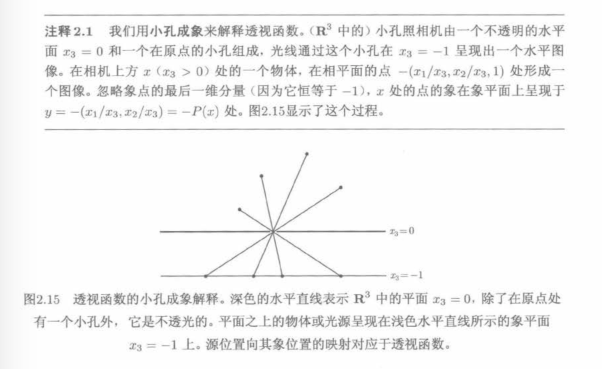
\includegraphics[width=1\linewidth]{pic/pic2_15}
	
	线性分式函数:由透视函数和仿射函数复合而成。函数\(f:R^n \to R^m\)
	
	\[f(x)=(Ax+b)/(c^Tx+d), dom f=\{x|c^Tx+d > 0\}\]
	
	\subsection{广义不等式}
	
	称锥\(K \subseteq R^n\)为正常锥,如果满足以下条件:
	1.K是凸的
	2.K是闭的
	3.K是实的,具有非空内部
	4.K是尖的,即不包含直线
	
	正常锥K可以用来定义广义不等式,即\(R^n\)上的偏序关系。
	
	\[x \preceq_K y \leftrightarrow y-x \in K\]
	
	严格的偏序关系
	
	\[x \prec_K y <==> y-x \in int K\]
	
	\textbf{最小与极小元}
	
	如果对于每个\(y \in S\),均有\(x \prec_K y\),称\(x \in S\)是S的最小元。如果一个集合有最小元,那么它们是唯一的。一个集合可以有多个极小元。
	
	元素\(x \in S\)是S中的一个最小元,当且仅当
	
	\[S \subseteq x+K\]
	
	x+K表示可以与x相比并且大于或等于x的所有元素
	
	元素\(x \in S\)是S中的极小元,当且仅当
	
	\[(x-K) \bigcap S = \{x\}\]
	
	x-K可以表示与x相比并且小于等于x的所有元素,它与S的唯一共同点是x
	
	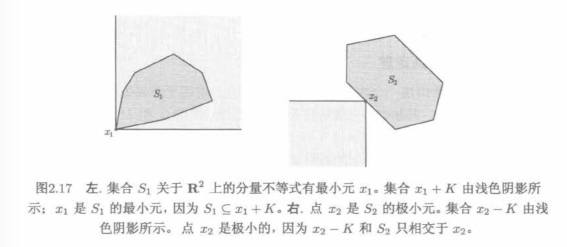
\includegraphics[width=1\linewidth]{pic/pic2_17}
	
	\textbf{补充:}最小(minimum):表示偏序集中其他的点都比它大;极小(minimal),表示该偏序集中没有比它更小的点,即该偏序集中的其他点要么比它大,要么和它不能够比较大小
	
	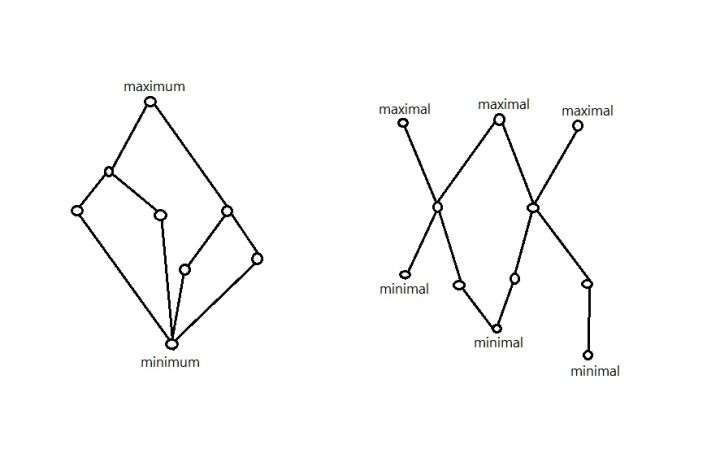
\includegraphics[width=1\linewidth]{pic/minimum_minimal}
	
	
	\subsection{分离与支撑超平面}
	
	\textbf{超平面分离定理}
	
	假设C和D是两个不相交的凸集,即\(C \bigcap D = \phi\),那么存在\(a \neq 0, b\)使得所有\(x \in C\)有\(a^Tx \leq b\),对于所有的\(x \in D\)有\(a^Tx \geq b\).超平面\(\{x|a^Tx = b\}\)成为集合C和D的分离超平面。
	
	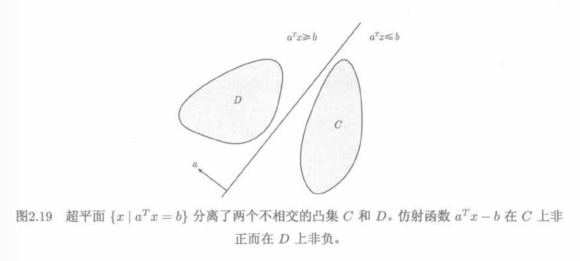
\includegraphics[width=1\linewidth]{pic/pic2_19}
	
	\textbf{支撑超平面}
	
	设\(C \subseteq R^n\)而\(x_0\)是其边界bdC上的一点,即
	
	\[x_0 \in bdC = clC \\\ intC\]
	
	如果\(a \neq 0\),并且对任意\(x \in C\)满足\(a^Tx \leq a^Tx_0\),那么称超平面\(\{x|a^Tx = a^Tx_0\}\)为集合C在点\(x_0\)处的支撑超平面。几何解释是超平面\(\{x|a^Tx = a^Tx_0\}\)与C相切与点\(x_0\),而且半空间\(\{x|a^Tx \leq a^Tx_0\}\)包含C。
	
	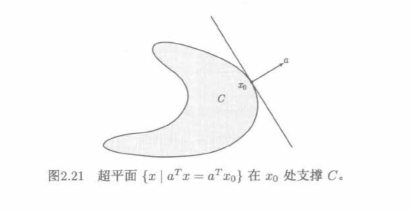
\includegraphics[width=1\linewidth]{pic/pic2_21}
	
	\subsection{对偶锥与广义不等式}
	
	令K为一个锥。集合
	
	\[K^*=\{y|x^Ty \geq 0 , \forall x \in K\}\]
	
	成为K的对偶锥。\(K^*\)是一个锥,并且总是凸的,即使K不是凸锥。
	
	从几何上看,\(y \in K^*\)当且仅当-y是K在原点的一个之称超平面的法线,如图
	
	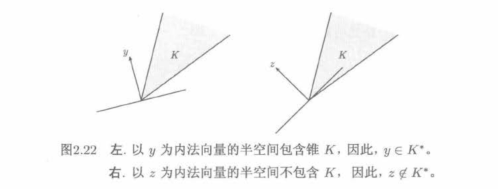
\includegraphics[width=1\linewidth]{pic/pic2_22}
	
	\textbf{广义不等式的对偶:}
	
	广义不等式\(\preceq_{K^*}\)为广义不等式\(\preceq_{K}\)的对偶
	
	
	
	
	
	
	
	
\end{document}